\documentclass[conference]{IEEEtran}
\IEEEoverridecommandlockouts
\usepackage{cite}
\usepackage{amsmath}
\usepackage{newtxtext,newtxmath}
\usepackage{algorithm}
\usepackage{algpseudocode}
\usepackage{graphicx}
\usepackage{booktabs}
\usepackage{multirow}
\usepackage{xcolor}
\usepackage{tikz}
\usetikzlibrary{positioning,arrows.meta,fit,backgrounds}
\usepackage[hidelinks]{hyperref}
\makeatletter
\newcommand{\linebreakand}{\end{@IEEEauthorhalign}\hfill\mbox{}\par\mbox{}\hfill\begin{@IEEEauthorhalign}}
\makeatother

\newcommand{\INR}{\text{\rupee}}
\DeclareRobustCommand{\rupee}{Rs.\,}

\begin{document}

\title{FinWise: Grounded Natural-Language Explanation of Personal Financial Transactions via Text-to-Analytics and Numeric Claim Verification}

\author{
\IEEEauthorblockN{Dhrumil Kadchha}
\IEEEauthorblockA{\textit{Dept. of CSE} \\
\textit{Dayananda Sagar University}\\
Bengaluru, India \\
dhrumilkadchha@gmail.com}
\and
\IEEEauthorblockN{Prathameshjee Sisodia}
\IEEEauthorblockA{\textit{Dept. of CSE} \\
\textit{Dayananda Sagar University}\\
Bengaluru, India \\
prathameshjeeesisodia@gmail.com}
\and
\IEEEauthorblockN{Pratyush Chauhan}
\IEEEauthorblockA{\textit{Dept. of CSE} \\
\textit{Dayananda Sagar University}\\
Bengaluru, India \\
pratyushchauhan099@gmail.com}
\linebreakand
\IEEEauthorblockN{Manu T J}
\IEEEauthorblockA{\textit{Dept. of CSE} \\
\textit{Dayananda Sagar University}\\
Bengaluru, India \\
manujogappa@gmail.com}
\and
\IEEEauthorblockN{Akmal Ahmad}
\IEEEauthorblockA{\textit{Dept. of CSE} \\
\textit{Dayananda Sagar University}\\
Bengaluru, India \\
akmalahmad2018@gmail.com}
}

\maketitle

\begin{abstract}
Bank statements list debits and credits but do not explain them, and a general-purpose large language model (LLM) given a raw statement tends to report totals that are not in the data. FinWise is a statement explainer for Indian bank exports (CSV, XLSX and PDF) in which numbers are produced only by deterministic code. The LLM is used for three narrow tasks: labelling merchants missing from an 86-pattern rule list, mapping a question to one of eleven typed analytics functions (\emph{Text-to-Analytics}), and wording the returned result. A \emph{Numeric Claim Verifier} parses every amount, percentage and ratio in the generated text and matches it against the computed values; the matched fraction is reported as the \emph{Grounded Faithfulness Score} (GFS). On 535 labelled transactions from three synthetic personas, the cache, rules and LLM categoriser scored 97.2\% accuracy (95\% CI 95.4--98.3\%) against 64.3\% for rules and 93.3\% for LLM-only labelling, using 6,832 instead of 13,319 tokens. A robust z-score detector with three domain rules recovered 15 of 15 planted anomalies (z-score baselines: at most 6). On 30 benchmark questions, Text-to-Analytics answered 90\% correctly against 25\% for prompting with the full statement (Fisher $p=3.6\times10^{-6}$), at about 1.25k instead of 6.3k tokens per question, and one verifier-triggered rewrite lifted numeric claim precision from 96.8\% to 100\%.
\end{abstract}

\begin{IEEEkeywords}
large language models, personal finance, explainable AI, hallucination mitigation, tool-augmented LLMs, anomaly detection, transaction categorisation
\end{IEEEkeywords}

%% =====================================================================
\section{Introduction}
India's UPI network settles several billion payments a month \cite{npci}. On a statement each payment collapses into a narration such as \texttt{UPI/DR/4123../SWIGGY/okaxis/Payment}, and a three-month export for one of our test users ran to 209 such rows. Budgeting apps group these rows by category and draw charts. They do not answer the follow-up a user actually has, for instance why October spending was 60\% higher than September, or whether two identical \rupee 649 Netflix debits on the same morning were a double charge.

Conversational LLMs \cite{brown2020} and finance-tuned variants \cite{wu2023bloomberggpt,yang2023fingpt,xie2023pixiu} can hold that dialogue, but three problems surfaced as soon as we tried. Arithmetic over long tables is unreliable \cite{chen2021finqa,zhu2021tatqa}; given the raw CSV, our first prototype reported a monthly total of about \rupee 2.7 lakh for a user who had spent well under \rupee 1 lakh, a case of the numeric hallucination surveyed in \cite{ji2023survey}. Narrations carry account references, UPI handles and friends' names, none of which should reach a hosted API. And three months of rows produced prompts above 6k tokens, which weakens recall of mid-context facts \cite{liu2024lost} and, for the largest statement, exceeded the per-request limit of the free Groq tier outright.

FinWise therefore restricts the model to language work and keeps arithmetic in code. Concretely, the paper contributes (i) an explain-then-verify loop in which computed facts are narrated by the LLM and every numeric claim is parsed and checked before display, with one feedback-driven rewrite on mismatch; (ii) the GFS, a faithfulness score for numeric claims that needs neither reference answers nor extra model calls; (iii) Text-to-Analytics, where the LLM fills arguments for one of eleven typed functions instead of reading the statement, so prompt size does not grow with $n$; (iv) a cache, rules and batched-LLM categoriser in the spirit of cost-aware cascades \cite{chen2023frugal}, with PII masked before any external call; and (v) an anomaly detector built on the modified z-score \cite{iglewicz1993}, evaluated with a per-component ablation. Sections~II--VIII cover related work, the problem definition, method, implementation, experimental setup, results and conclusions.

%% =====================================================================
\section{Related Work}
\textbf{Finance-oriented LLMs.} BloombergGPT \cite{wu2023bloomberggpt} and FinGPT \cite{yang2023fingpt} adapt language models to financial text, and PIXIU \cite{xie2023pixiu} and FLUE \cite{shah2022flue} supply benchmarks for them. Their focus is news, filings and market sentiment. None of them deals with an individual's transactions, and none restricts what numbers the model is allowed to state.

\textbf{Numerical reasoning and tools.} FinQA \cite{chen2021finqa} and TAT-QA \cite{zhu2021tatqa} show that multi-step reasoning over financial tables remains hard even for large models. One remedy is to have the model write a program and execute it, as in PAL \cite{gao2023pal} and Program-of-Thoughts \cite{chen2023pot}; another lets the model call tools while it reasons, as in ReAct \cite{yao2023react} and Toolformer \cite{schick2023toolformer}. Text-to-SQL systems \cite{yu2018spider,rajkumar2022sql} apply the same idea to database queries. FinWise takes the tool-calling route but limits it to eleven functions with typed arguments. The model never emits code, so nothing has to be sandboxed, and each answer can be traced to a single function call and its inputs.

\textbf{Detecting hallucination.} Ji et al.\ \cite{ji2023survey} classify hallucination types across generation tasks. Detection methods differ mainly in what they compare against: SelfCheckGPT \cite{manakul2023selfcheck} measures agreement among several sampled answers, FActScore \cite{min2023factscore} checks atomic facts against a knowledge source, and retrieval-augmented generation \cite{lewis2020rag} conditions the output on retrieved passages. The FinWise verifier resembles FActScore at the level of individual claims, but its claims are numbers only, its reference set is computed from the user's own data rather than retrieved, and the check itself is a regular-expression parser plus a tolerance test, so no extra model call is made.

\textbf{Outliers and cost.} Chandola et al.\ \cite{chandola2009anomaly} review classical anomaly detection. We start from the modified z-score of Iglewicz and Hoaglin \cite{iglewicz1993}, whose median and MAD are not distorted by the outliers being sought, and add rules specific to spending data. FrugalGPT \cite{chen2023frugal} argues for trying cheap predictors before expensive ones, which is the ordering our categoriser follows.


%% =====================================================================
\section{Problem Formulation}
We model a statement as a sequence $D=\{t_i\}_{i=1}^{n}$, where each $t_i=(d_i, s_i, a_i, \delta_i)$ holds a date, the raw narration, an amount $a_i>0$ and a direction $\delta_i\in\{\text{debit},\text{credit}\}$. There is a fixed set $\mathcal{K}$ of 15 categories, and $m(s_i)$ denotes the merchant we extract from a narration. Three tasks follow.

\textbf{T1, categorisation.} Find $f: (s_i,\delta_i,a_i)\mapsto k\in\mathcal{K}$ with high accuracy while sending as few tokens as possible to an external model. Only a masked version $\mu(s_i)$ of the narration may leave the system.

\textbf{T2, anomaly explanation.} Identify a subset $A\subseteq D$ that a user would find unusual and, for each $t\in A$, give a reason and a suggested action that agree with $D$.

\textbf{T3, grounded question answering.} For a question $q$, return an answer $y$ that is correct and also \emph{numerically faithful}. Writing $C(y)$ for the numeric claims in $y$ and $F$ for the facts computable from $D$, we require each claim to match some fact within a tolerance $\tau$:
\begin{equation}
\forall c\in C(y)\;\; \exists f\in F:\; \lvert v(c)-f\rvert \le \tau(c,f).
\end{equation}
We measure how far an answer satisfies this with
\begin{equation}
\mathrm{GFS}(y)=\frac{\lvert\{c\in C(y): c \text{ supported by } F\}\rvert}{\lvert C(y)\rvert},
\end{equation}
with $\mathrm{GFS}(y)=1$ when $C(y)=\emptyset$.

%% =====================================================================
\section{Proposed Methodology}
\begin{figure}[t]
\centering
\resizebox{\columnwidth}{!}{%
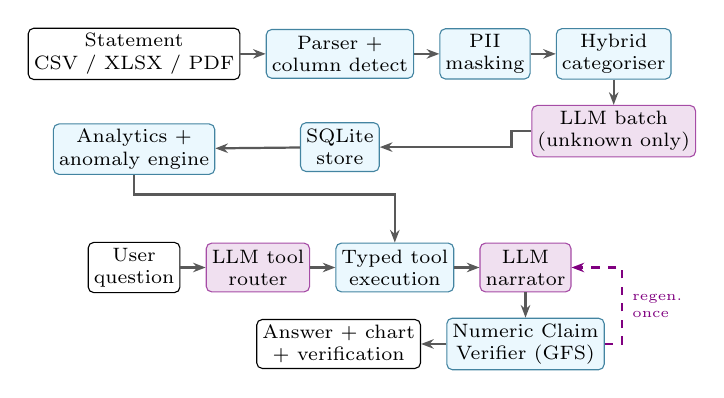
\begin{tikzpicture}[
  box/.style={draw, rounded corners=2pt, align=center, font=\scriptsize, minimum height=0.62cm, inner sep=2pt, fill=white},
  llm/.style={box, fill=violet!12, draw=violet!70},
  det/.style={box, fill=cyan!8, draw=cyan!60!black},
  arr/.style={-{Stealth[length=1.6mm]}, thick, gray!70!black},
  node distance=0.32cm and 0.32cm]
\node[box] (up) {Statement\\CSV / XLSX / PDF};
\node[det, right=of up] (ing) {Parser +\\column detect};
\node[det, right=of ing] (pii) {PII\\masking};
\node[det, right=of pii] (cat) {Hybrid\\categoriser};
\node[llm, below=of cat] (lcat) {LLM batch\\(unknown only)};
\node[det, below=0.55cm of ing] (db) {SQLite\\store};
\node[det, below=0.55cm of up] (ana) {Analytics +\\anomaly engine};
\node[box, below=0.85cm of ana] (q) {User\\question};
\node[llm, right=of q] (route) {LLM tool\\router};
\node[det, right=of route] (tool) {Typed tool\\execution};
\node[llm, right=of tool] (narr) {LLM\\narrator};
\node[det, below=of narr] (ver) {Numeric Claim\\Verifier (GFS)};
\node[box, left=of ver] (ui) {Answer + chart\\+ verification};
\draw[arr] (up)--(ing); \draw[arr] (ing)--(pii); \draw[arr] (pii)--(cat);
\draw[arr] (cat)--(lcat); \draw[arr] (lcat.west) -- ++(-0.25,0) |- (db.east);
\draw[arr] (db)--(ana); \draw[arr] (q)--(route); \draw[arr] (route)--(tool);
\draw[arr] (ana.south) -- ++(0,-0.25) -| (tool.north); \draw[arr] (tool)--(narr);
\draw[arr] (narr)--(ver); \draw[arr] (ver)--(ui);
\draw[arr, dashed, violet] (ver.east) -- ++(0.22,0) |- node[pos=0.25, right, font=\tiny, align=left]{regen.\\once} (narr.east);
\end{tikzpicture}}
\caption{FinWise architecture. Deterministic components (cyan) compute every number; LLM components (violet) only classify unknown merchants, select tools and narrate verified facts.}
\label{fig:arch}
\end{figure}

Fig.~\ref{fig:arch} gives an overview. The upper path runs once when a statement is uploaded; the lower path runs for every question.

\subsection{Ingestion and Privacy Masking}
No two Indian banks seem to export statements the same way. Some put banner rows above the header, some use \emph{Narration} and others \emph{Particulars}, and amounts arrive as separate debit and credit columns, as signed numbers, or as an amount with a Dr/Cr flag. The parser looks for the real header row, matches columns against a list of synonyms and handles all three amount layouts. PDFs are read with \texttt{pdfplumber}, with a line-by-line regular-expression fallback for statements that have no ruled table, and dates are parsed day-first. To get a merchant name we split the narration by channel (the fourth field for UPI, the third for NEFT and IMPS, the second for ACH, the text after the card number for POS) and strip legal suffixes, month names and digits.

Masking is applied before categorisation, so no later stage sees unmasked text. The function $\mu$ replaces e-mail addresses, UPI handles, PAN numbers, phone numbers and any digit run longer than five, and rewrites a payee as \texttt{[PERSON]} when its first token appears in a list of 70 common Indian given names. Apart from protecting names, the token turned out to be a strong \emph{Transfers} cue for the LLM. On the evaluation set $\mu$ redacted reference numbers in 518 of 535 narrations and replaced 33 payee names.

\subsection{Cost-Aware Hybrid Categorisation}
Categorisation is a cascade. A transaction is first looked up in a merchant cache keyed on $(m,\delta)$ that stores earlier decisions and user corrections. Unknown merchants are matched against 86 regular-expression patterns for well-known Indian brands, billers and keywords such as \emph{salary} and \emph{rent} (income patterns only fire on credits). Whatever remains goes to the LLM once per distinct $(m,\delta)$ pair, as one masked example with direction and rounded amount, in batches of $B=30$. The prompt holds the 15 category names, nine disambiguation rules (fuel stations and metro cards belong to \emph{Transport}, gyms and streaming to \emph{Subscriptions}, and so on) and three few-shot examples \cite{brown2020}; the reply is requested in JSON mode at temperature 0. Labels outside $\mathcal{K}$ are discarded and the item falls back to a heuristic. The number of model calls is $\lceil |M_u|/B\rceil$, where $M_u$ is the set of merchants unknown to the rules, independent of $n$; on a second upload of the same statement every merchant is served from the cache or the rules and no LLM call is made.

\subsection{Context-Aware Anomaly Detection}
For each category $c$ we take the debit amounts $X_c$ (rent, EMIs, transfers and cash withdrawals are left out) and their median $\tilde{m}_c$, and compute the robust z-score
\begin{equation}
z(x)=\frac{0.6745\,(x-\tilde{m}_c)}{\mathrm{MAD}_c},\qquad \mathrm{MAD}_c=\operatorname{median}_{y\in X_c}\lvert y-\tilde{m}_c\rvert ,
\end{equation}
A transaction counts as a \emph{spike} when $z(x)>3.5$, $x\ge 2.5\,\tilde{m}_c$ and $x\ge$ \rupee 500, provided the category has at least five past debits \cite{iglewicz1993}. Median and MAD are used instead of mean and standard deviation because a single large purchase pulls the mean towards itself and hides its own deviation, the masking effect described in \cite{chandola2009anomaly}.

Our first version of the detector raised a stream of false alarms in \emph{Transport}. The reason was that the category mixes \rupee 150 cab rides with \rupee 2,000 fuel fills, so every refuelling looked extreme. We fixed this with what we call habitual-merchant suppression: if a merchant has been paid at least three times and the amount is no more than twice that merchant's median $\tilde{m}_m$, the payment is left alone. Running the same robust test within a single merchant (at least four payments, $x\ge 3\,\tilde{m}_m$) catches the opposite case, such as a \rupee 2,380 cab ride from someone whose rides usually cost \rupee 373. Two further rules cover anomalies that are not statistical outliers at all: a \emph{duplicate charge} (same merchant, same amount, within a day) and a \emph{new high-value merchant} (first seen in the latest month, with $x\ge\max(\text{\rupee}5000, P_{95})$). Every flag carries a sentence with the exact computed values, for instance ``\rupee 4,250 at Swiggy is 8.9$\times$ your usual \rupee 475'', and that sentence is what the LLM later explains. The whole procedure runs in $O(n\log n)$ time.

\subsection{Text-to-Analytics Question Answering}
Table~\ref{tab:tools} lists the functions. The routing prompt (about 650 tokens) holds their signatures, the months present in $D$ and the category names; the LLM returns \texttt{\{tool, args\}} in JSON mode at temperature 0. This follows the tool-use pattern of \cite{yao2023react,schick2023toolformer}, except that the menu is closed. The last four chat turns are appended so that an elliptical follow-up (``and September?'') inherits the previous function. Arguments are normalised before execution: \emph{latest} and \emph{previous} map to concrete months, and free-text categories are fuzzy-matched (``food'' to \emph{Food \& Dining}). Execution returns a result object $R$ and an optional chart specification. Because $D$ is never placed in the prompt, a question costs two model calls, three with a rewrite, for any $n$, which also sidesteps the long-context degradation reported in \cite{liu2024lost}.

\begin{table}[t]
\caption{Typed analytics tools available to the router}
\label{tab:tools}
\centering
\resizebox{\columnwidth}{!}{%
\begin{tabular}{@{}lll@{}}
\toprule
Tool & Arguments & Returns \\
\midrule
\texttt{spending\_summary} & month & totals, savings rate, by category \\
\texttt{category\_spend} & category, month & total, mean, max, top merchants \\
\texttt{top\_merchants} & $n$, month, category & ranked merchants \\
\texttt{compare\_months} & month$_a$, month$_b$ & per-category change \\
\texttt{find\_transactions} & text, category, range & matching rows, total \\
\texttt{subscriptions} & -- & services, monthly/annual cost \\
\texttt{upcoming\_bills} & -- & payments due in 30 days \\
\texttt{unusual\_expenses} & -- & anomalies with reasons \\
\texttt{budget\_suggestion} & -- & 50/30/20 targets vs.\ actual \\
\texttt{health\_score} & -- & score, five components \\
\texttt{spending\_patterns} & -- & weekday/weekend, recurring \\
\bottomrule
\end{tabular}}
\end{table}

\subsection{Grounded Explain-then-Verify}
The narration prompt passes $q$ and $R$ at temperature 0.3 with four constraints: copy figures verbatim, round to whole rupees, derive nothing, and say so when $R$ lacks the answer. The verifier first deletes dates and years, then extracts three claim types with regular expressions: amounts (a currency marker before the number, Indian scale words such as \emph{k}, \emph{lakh} and \emph{crore}, or a bare number of at least 1,000 or with digit grouping), percentages (\%) and ratios ($\times$, \emph{x}, \emph{times}). $F$ is the set of numbers in $R$, $a$ and $q$, with ratios also added in percent form. Tolerances are $\max(1, 0.01f)$ for amounts, widened to half a unit of the stated precision for scaled forms (``\rupee 1.2 lakh'' accepts 1.15--1.25 lakh), 0.6 points for percentages and 0.15 for ratios. In effect this is atomic-fact checking \cite{min2023factscore} restricted to numbers and run against computed rather than retrieved references. Algorithm~\ref{alg:gev} gives the loop; the same routine checks the anomaly explanations ($F$ = anomaly facts) and the five dashboard insights ($F$ = a statement-level fact sheet) at $O(|C(y)|\,|F|)$ cost, with no model call.

\begin{algorithm}[t]
\caption{Grounded Explain-then-Verify}\label{alg:gev}
\begin{algorithmic}[1]
\Require question $q$, transactions $D$, tools $\mathcal{T}$, retries $K{=}1$
\State $(t,a) \gets \textsc{LLM-Route}(q,\mathcal{T})$ \Comment{JSON mode}
\State $R \gets t(D,a)$ \Comment{deterministic}
\State $y \gets \textsc{LLM-Narrate}(q,R)$; \ $F \gets \mathrm{nums}(R)\cup\mathrm{nums}(a)\cup\mathrm{nums}(q)$
\For{$k=1$ \textbf{to} $K$}
  \State $U \gets \{c\in C(y): c \text{ unsupported by } F\}$
  \If{$U=\emptyset$} \textbf{break} \EndIf
  \State $y \gets \textsc{LLM-Narrate}(q,R,\text{feedback}=U)$
\EndFor
\State \Return $y$, $\mathrm{GFS}(y)$, $U$ \Comment{unresolved claims are flagged}
\end{algorithmic}
\end{algorithm}

\subsection{Patterns and Financial Health Score}
Recurring payments drive the subscription and upcoming-bill features. We call a merchant recurring when it shows up in at least $M-1$ of the $M$ months, with a median gap between payments of 20--40 days and no more than 1.5 payments a month. The amounts must also be steady: a coefficient of variation of at most 0.35 for bills, subscriptions, rent and EMIs, and at most 0.03 (with a payment in every month) for anything else. That second, much stricter threshold was added after an early version listed a favourite coffee shop as a subscription. Next due date = last payment + median gap. Table~\ref{tab:health} defines the 0--100 health score as a sum of five clipped terms, and the budget function applies the 50/30/20 split of needs, wants and savings \cite{warren2005} to average monthly income.

\begin{table}[t]
\caption{Financial health score components (total 100)}
\label{tab:health}
\centering
\resizebox{\columnwidth}{!}{%
\begin{tabular}{@{}llc@{}}
\toprule
Component & Formula (clipped to $[0,\max]$) & Max \\
\midrule
Savings rate $r$ (\%) & $40\,r/30$ & 40 \\
Discretionary share $d$ (\%) & $20-0.5\max(0,d-30)$ & 20 \\
Subscriptions $u$ (\% of income) & $15-3\max(0,u-3)$ & 15 \\
Unusual expenses $n_a$ & $10-1.5\,n_a$ & 10 \\
Stability (CV of monthly spend) & $15-30\,\mathrm{CV}$ & 15 \\
\bottomrule
\multicolumn{3}{@{}l}{\footnotesize Labels: $\ge$80 Excellent, $\ge$65 Good, $\ge$45 Fair, otherwise Needs attention.}
\end{tabular}}
\end{table}

%% =====================================================================
\section{Implementation}
The backend uses Python 3.12, FastAPI, pandas \cite{mckinney2010} and SQLite. Upload, dashboard, transaction, insight and anomaly endpoints are plain REST; chat is streamed over Server-Sent Events as three event types (\texttt{tool}, \texttt{token}, \texttt{done}), the last carrying the verifier report. The LLM client targets the OpenAI-compatible chat API, so Groq and Gemini differ only in base URL and key. Llama~3.3 was our original choice but was not enabled for our free Groq key, so all runs use \texttt{gpt-oss-120b} \cite{openai2025gptoss} with reasoning effort set to low. The client adds JSON mode, exponential back-off on HTTP 429, a SHA-256-keyed response cache and optional throttling; with no key configured it degrades to rules and templates. The React/TypeScript front end shows a dashboard, a transaction table with inline re-labelling, an insights page and a chat view. Each AI-written paragraph carries a ``Verified $\cdot$ $k$ numbers'' badge, and each label shows its source (rule, LLM or user).

%% =====================================================================
\section{Experimental Setup}
\textbf{Data.} We know of no public, labelled corpus of personal bank statements. We wrote a generator (seeds 2026--2028) for three personas over August--October 2026 (Table~\ref{tab:data}). Narrations follow UPI, NEFT, POS and ACH layouts as they appear in HDFC- and SBI-style exports, and each persona is written to a different file format. Of the 88 merchants, 46 are local businesses (cafes, kirana stores, clinics, bike rentals) kept out of the rule list on purpose. The class distribution is skewed, led by Food \& Dining (168), Transport (102) and Groceries (64). Fifteen anomalies were inserted: nine spikes, three duplicate charges and three large first-time payments.

\begin{table}[t]
\caption{Evaluation dataset}
\label{tab:data}
\centering
\resizebox{\columnwidth}{!}{%
\begin{tabular}{@{}lccccc@{}}
\toprule
Persona & Format & Txns & Merchants & Anomalies & Profile \\
\midrule
Aarav & CSV & 209 & 58 & 6 & salaried, renter \\
Priya & XLSX & 166 & 59 & 5 & salaried, car EMI \\
Rohan & PDF & 160 & 45 & 4 & freelancer \\
\midrule
Total & 3 formats & 535 & 88 & 15 & 14 categories \\
\bottomrule
\end{tabular}}
\end{table}

\textbf{Experiments.} In E1 we compare three ways of categorising: rules only, the LLM for every transaction, and our hybrid. We report accuracy with 95\% Wilson intervals \cite{wilson1927}, macro-F1 computed with scikit-learn \cite{pedregosa2011}, the number of model calls and tokens. In E2 we compare a global z-score ($z>3$), a per-category z-score and our detector, once with the true categories and once with the categories the hybrid predicted, and then remove one component of our detector at a time. In E3 we ask ten questions per person, 30 in all (for example, ``By how much did my total spending change from September to October?''), with reference answers computed from the true labels. Three strategies answer them: (a) putting the whole masked statement into the prompt as CSV, which we refer to as context stuffing; (b) Text-to-Analytics without checking; and (c) Text-to-Analytics with the verifier. An answer is counted as correct if it states the expected value within 1\%, or 0.6 points for percentages. We also report claim precision (supported claims over all claims), mean GFS and the share of answers with GFS of 1, and use Fisher's exact test \cite{fisher1925} to compare accuracies. Every run used \texttt{gpt-oss-120b} on the free Groq tier.

%% =====================================================================
%% =====================================================================
\section{Results and Discussion}
\subsection{Categorisation (E1)}
Table~\ref{tab:cat} shows the expected pattern for rules: they never get a well-known brand wrong but have nothing to say about the long tail, which ends up as \emph{Other}, so accuracy stops at 64.3\%. Sending every transaction to the model lifts accuracy to 93.3\% but costs 13.3k tokens, and, somewhat to our surprise, the model also got a few easy merchants wrong that the rules had handled, which pulls macro-F1 down to 0.858. The hybrid reaches 97.2\% with a macro-F1 of 0.967. Its confidence interval (95.4--98.3\%) does not overlap with that of the LLM-only run (90.8--95.1\%), and it needs half as many calls and 49\% fewer tokens. Looking inside the hybrid, all 344 transactions labelled by rules were correct, and the 191 labelled by the model, covering 46 distinct merchants, were 92.1\% correct.

\begin{table}[t]
\caption{E1: Transaction categorisation (535 txns, 15 classes)}
\label{tab:cat}
\centering
\resizebox{\columnwidth}{!}{%
\begin{tabular}{@{}lcccccc@{}}
\toprule
Mode & Acc. & 95\% CI & Macro-F1 & Calls & Tokens & Txns via LLM \\
\midrule
Rules only & 0.643 & [0.602, 0.682] & 0.676 & 0 & 0 & 0 \\
LLM only & 0.933 & [0.908, 0.951] & 0.858 & 6 & 13{,}319 & 535 \\
\textbf{Hybrid (ours)} & \textbf{0.972} & [0.954, 0.983] & \textbf{0.967} & 3 & 6{,}832 & 191 \\
\bottomrule
\end{tabular}}
\end{table}

Per-category F1 is listed in Table~\ref{tab:perclass}; nine categories are error-free. All 15 errors come from six long-tail merchants: a kirana store and an e-bike rental labelled \emph{Shopping} (4 transactions each), a rental platform's monthly debit labelled \emph{Subscriptions} (3), a sweets-and-snacks chain labelled \emph{Groceries} (2), and one error each for an EV cab operator and an eyewear retailer. In the application each of these is fixed permanently by a single user correction written to the cache.

\begin{table}[t]
\caption{Per-category F1 of the hybrid categoriser (support in brackets)}
\label{tab:perclass}
\centering
\resizebox{\columnwidth}{!}{%
\begin{tabular}{@{}lc|lc@{}}
\toprule
Category & F1 & Category & F1 \\
\midrule
Food \& Dining (168) & 0.994 & Bills \& Utilities (24) & 1.000 \\
Transport (102) & 0.975 & Income (16) & 1.000 \\
Groceries (64) & 0.952 & Entertainment (16) & 1.000 \\
Shopping (42) & 0.891 & Health (14) & 0.966 \\
Subscriptions (38) & 0.962 & Rent \& Housing (9) & 0.800 \\
Transfers (27) & 1.000 & EMI, Cash, Education (15) & 1.000 \\
\bottomrule
\end{tabular}}
\end{table}

\subsection{Anomaly Detection (E2)}
Both z-score baselines miss most of the planted anomalies, with recall of 0.33--0.40 (Table~\ref{tab:anom}). A large outlier inflates the mean and standard deviation meant to expose it \cite{iglewicz1993}, and a duplicate charge is not an outlier at all. Our detector finds all 15 (recall 95\% CI 0.80--1.00; Fisher $p=7\times10^{-4}$ against the global z-score). On predicted instead of true categories two false alarms appear, because a few mislabelled transactions shift the category medians, and F1 drops to 0.94.

\begin{table}[t]
\caption{E2: Anomaly detection (15 planted anomalies)}
\label{tab:anom}
\centering
\resizebox{\columnwidth}{!}{%
\begin{tabular}{@{}llcccc@{}}
\toprule
Categories & Method & TP/FP/FN & P & R & F1 \\
\midrule
\multirow{3}{*}{Ground truth} & Global $z$ & 6/0/9 & 1.000 & 0.400 & 0.571 \\
 & Category $z$ & 5/1/10 & 0.833 & 0.333 & 0.476 \\
 & \textbf{FinWise} & 15/0/0 & \textbf{1.000} & \textbf{1.000} & \textbf{1.000} \\
\midrule
\multirow{3}{*}{Predicted} & Global $z$ & 5/3/10 & 0.625 & 0.333 & 0.435 \\
 & Category $z$ & 6/1/9 & 0.857 & 0.400 & 0.545 \\
 & \textbf{FinWise} & 15/2/0 & \textbf{0.882} & \textbf{1.000} & \textbf{0.938} \\
\bottomrule
\end{tabular}}
\end{table}

Table~\ref{tab:abl} removes one component at a time. Dropping habitual-merchant suppression adds six false positives, all refuelling payments, which is the failure that led us to add the rule. Without the minimum-history guard two one-off course fees are flagged; without the duplicate rule the three double charges are missed (recall 0.80). The merchant-level and new-merchant rules leave the counts unchanged here but yield more specific reason strings. Table~\ref{tab:explain} lists generated explanations for the Aarav statement: type and figures come from the detector, cause and action from the LLM, and every number passed verification.

\begin{table}[t]
\caption{E2b: Detector ablation (ground-truth categories)}
\label{tab:abl}
\centering
\resizebox{\columnwidth}{!}{%
\begin{tabular}{@{}lcccc@{}}
\toprule
Component removed & TP/FP/FN & P & R & F1 \\
\midrule
None (full detector) & 15/0/0 & 1.000 & 1.000 & 1.000 \\
Habitual-merchant suppression & 15/6/0 & 0.714 & 1.000 & 0.833 \\
Minimum-history guard & 15/2/0 & 0.882 & 1.000 & 0.938 \\
Duplicate-charge rule & 12/0/3 & 1.000 & 0.800 & 0.889 \\
Merchant-level spike & 15/0/0 & 1.000 & 1.000 & 1.000 \\
New-merchant rule & 15/0/0 & 1.000 & 1.000 & 1.000 \\
\bottomrule
\end{tabular}}
\end{table}

\begin{table}[t]
\caption{Generated anomaly explanations (Aarav statement, abridged)}
\label{tab:explain}
\centering
\footnotesize
\begin{tabular}{@{}p{0.17\columnwidth}p{0.75\columnwidth}@{}}
\toprule
Type & Computed reason $\rightarrow$ generated explanation / action \\
\midrule
Duplicate & Rs.\,649 charged twice at Netflix on 02 Oct $\rightarrow$ ``indicates a duplicate transaction; request a refund from Netflix support.'' \\
Spike (merchant) & Rs.\,2,380 at Uber is 6.4$\times$ the usual Rs.\,373 $\rightarrow$ ``check the receipt for distance or surge pricing.'' \\
Spike (category) & Rs.\,4,860 electricity bill is 4.6$\times$ the median utility spend of Rs.\,1,059 $\rightarrow$ ``inspect the bill for meter-reading errors.'' \\
New merchant & First payment to Croma, Rs.\,18,990, above 95\% of expenses $\rightarrow$ ``verify the purchase; set a limit for new merchants.'' \\
\bottomrule
\end{tabular}
\end{table}

\subsection{Question Answering and Faithfulness (E3)}
Table~\ref{tab:qa} has the main result. For the 209-row statement all ten full-statement prompts were rejected by the provider for exceeding the per-request token limit. On the remaining 20 questions, full-statement prompting answered 25\% correctly (16.7\% if rejections count as failures). Its failures were of two kinds: refusals (``I can't calculate that total from the data provided'') and confident wrong totals, such as about \rupee 2.71 lakh for one month's spending, consistent with the long-context \cite{liu2024lost} and table-arithmetic \cite{chen2021finqa} weaknesses noted earlier. Only 51.7\% of its numeric claims matched a fact. Text-to-Analytics answered 90\% correctly (95\% CI 74--97\%; Fisher $p=3.6\times10^{-6}$), with 96.8\% supported claims and about 1.25k tokens per question (roughly 690 for routing and 560 for narration) against 6.3k. The verifier flagged one unsupported value, a ``10\%'' absent from $R$, and the rewrite removed it; all 30 final answers had GFS $=1$, for one extra call in 30.

\begin{table}[t]
\caption{E3: QA correctness and numeric faithfulness}
\label{tab:qa}
\centering
\resizebox{\columnwidth}{!}{%
\begin{tabular}{@{}lcccccc@{}}
\toprule
Strategy & $N$ & Acc. & 95\% CI & Claim prec. & Mean GFS & Tokens/q \\
\midrule
Context stuffing & 20$^\dagger$ & 0.250 & [0.11, 0.47] & 0.517 & 0.631 & 6{,}334 \\
Text-to-Analytics & 30 & 0.900 & [0.74, 0.97] & 0.968 & 0.983 & $\approx$1{,}250 \\
\textbf{+ Verifier (ours)} & 30 & \textbf{0.900} & [0.74, 0.97] & \textbf{1.000} & \textbf{1.000} & +3.3\% calls \\
\bottomrule
\multicolumn{7}{@{}l}{\footnotesize $^\dagger$The other 10 of 30 requests exceeded the API's per-request token limit.}
\end{tabular}}
\end{table}


\textbf{An example.} For ``Why was October so expensive compared to September?'' the router chose \texttt{compare\_months(previous, latest)}. The answer reported total spend rising from \rupee 62,229 to \rupee 99,680 (+60.18\%), mainly from Shopping (\rupee 10,717 to \rupee 40,656), and proposed a weekly shopping cap; 29 of 29 numbers matched $R$.

\textbf{Errors.} All three wrong Text-to-Analytics answers had GFS $=1$. They repeated the computed totals correctly, but those totals inherited E1 labelling errors (the kirana store and snack chain in two grocery totals, the rental platform in one subscription total). The verifier certifies agreement between text and computation, not the correctness of the labels feeding the computation. The interface narrows this gap by showing each label's source and persisting one-click corrections.

\textbf{Cost.} Spend grows with the number of questions and of unseen merchants, not with $n$. A 12-month statement (about 800 rows) would still cost about 1.25k tokens per question, against roughly 4$\times$ the 6.3k observed for full-statement prompts, which would also break the free-tier request cap.

\textbf{Lessons.} Eleven typed functions covered all 30 benchmark questions, and malformed arguments were rare and easy to catch. Verification is cheap enough to run on every reply. Putting rules ahead of the LLM improved accuracy as well as cost, since all 344 rule labels were correct.

\textbf{Limitations.} The statements are synthetic and detector thresholds were set on the same personas, so F1 $=1.0$ on true categories is optimistic. The 30 questions are templated, only numeric claims are verified (``your largest expense'' is not), and a single LLM was tested; latency is omitted because requests were throttled for the free tier. Seeds, prompts, scripts and raw outputs are kept with the code so that every figure can be regenerated.

%% =====================================================================
\section{Conclusion and Future Work}
FinWise keeps the LLM on language tasks (reading a question, naming an unfamiliar merchant, wording a result) and keeps every calculation in code, with each emitted number checked against the computation. On 535 labelled transactions this gave 97.2\% categorisation accuracy at half the LLM-only token cost, recovered all 15 planted anomalies, and raised question-answering accuracy from 25\% to 90\% with no unsupported numbers in the final answers. Next steps are an evaluation on consented real statements obtained through India's Account Aggregator framework \cite{rbi2016aa}, together with a user study of trust and comprehension, support for Hindi and code-mixed questions, verification of non-numeric claims, and small on-device models so that statements never leave the user's phone.

\section*{Acknowledgment}
This work was carried out as an LLM mini project in the Department of Computer Science and Engineering, Dayananda Sagar University, Bengaluru, whose laboratory facilities we used throughout.

\begin{thebibliography}{00}
\bibitem{npci} National Payments Corporation of India, ``UPI product statistics,'' 2025. [Online]. Available: https://www.npci.org.in/what-we-do/upi/product-statistics
\bibitem{brown2020} T. B. Brown \emph{et al.}, ``Language models are few-shot learners,'' in \emph{Proc. NeurIPS}, 2020, pp. 1877--1901.
\bibitem{wu2023bloomberggpt} S. Wu \emph{et al.}, ``BloombergGPT: A large language model for finance,'' arXiv:2303.17564, 2023.
\bibitem{yang2023fingpt} H. Yang, X.-Y. Liu, and C. D. Wang, ``FinGPT: Open-source financial large language models,'' arXiv:2306.06031, 2023.
\bibitem{xie2023pixiu} Q. Xie \emph{et al.}, ``PIXIU: A large language model, instruction data and evaluation benchmark for finance,'' in \emph{Proc. NeurIPS Datasets and Benchmarks Track}, 2023.
\bibitem{chen2021finqa} Z. Chen \emph{et al.}, ``FinQA: A dataset of numerical reasoning over financial data,'' in \emph{Proc. EMNLP}, 2021, pp. 3697--3711.
\bibitem{zhu2021tatqa} F. Zhu \emph{et al.}, ``TAT-QA: A question answering benchmark on a hybrid of tabular and textual content in finance,'' in \emph{Proc. ACL}, 2021, pp. 3277--3287.
\bibitem{ji2023survey} Z. Ji \emph{et al.}, ``Survey of hallucination in natural language generation,'' \emph{ACM Comput. Surv.}, vol. 55, no. 12, pp. 1--38, 2023.
\bibitem{liu2024lost} N. F. Liu \emph{et al.}, ``Lost in the middle: How language models use long contexts,'' \emph{Trans. Assoc. Comput. Linguistics}, vol. 12, pp. 157--173, 2024.
\bibitem{chen2023frugal} L. Chen, M. Zaharia, and J. Zou, ``FrugalGPT: How to use large language models while reducing cost and improving performance,'' arXiv:2305.05176, 2023.
\bibitem{iglewicz1993} B. Iglewicz and D. C. Hoaglin, \emph{How to Detect and Handle Outliers}. Milwaukee, WI, USA: ASQC Quality Press, 1993.
\bibitem{shah2022flue} R. S. Shah \emph{et al.}, ``When FLUE meets FLANG: Benchmarks and large pretrained language model for financial domain,'' in \emph{Proc. EMNLP}, 2022, pp. 2322--2335.
\bibitem{gao2023pal} L. Gao \emph{et al.}, ``PAL: Program-aided language models,'' in \emph{Proc. ICML}, 2023, pp. 10764--10799.
\bibitem{chen2023pot} W. Chen, X. Ma, X. Wang, and W. W. Cohen, ``Program of thoughts prompting: Disentangling computation from reasoning for numerical reasoning tasks,'' \emph{Trans. Mach. Learn. Res.}, 2023.
\bibitem{yao2023react} S. Yao \emph{et al.}, ``ReAct: Synergizing reasoning and acting in language models,'' in \emph{Proc. ICLR}, 2023.
\bibitem{schick2023toolformer} T. Schick \emph{et al.}, ``Toolformer: Language models can teach themselves to use tools,'' in \emph{Proc. NeurIPS}, 2023.
\bibitem{yu2018spider} T. Yu \emph{et al.}, ``Spider: A large-scale human-labeled dataset for complex and cross-domain semantic parsing and text-to-SQL task,'' in \emph{Proc. EMNLP}, 2018, pp. 3911--3921.
\bibitem{rajkumar2022sql} N. Rajkumar, R. Li, and D. Bahdanau, ``Evaluating the text-to-SQL capabilities of large language models,'' arXiv:2204.00498, 2022.
\bibitem{manakul2023selfcheck} P. Manakul, A. Liusie, and M. J. F. Gales, ``SelfCheckGPT: Zero-resource black-box hallucination detection for generative large language models,'' in \emph{Proc. EMNLP}, 2023, pp. 9004--9017.
\bibitem{min2023factscore} S. Min \emph{et al.}, ``FActScore: Fine-grained atomic evaluation of factual precision in long form text generation,'' in \emph{Proc. EMNLP}, 2023, pp. 12076--12100.
\bibitem{lewis2020rag} P. Lewis \emph{et al.}, ``Retrieval-augmented generation for knowledge-intensive NLP tasks,'' in \emph{Proc. NeurIPS}, 2020, pp. 9459--9474.
\bibitem{chandola2009anomaly} V. Chandola, A. Banerjee, and V. Kumar, ``Anomaly detection: A survey,'' \emph{ACM Comput. Surv.}, vol. 41, no. 3, pp. 1--58, 2009.
\bibitem{warren2005} E. Warren and A. W. Tyagi, \emph{All Your Worth: The Ultimate Lifetime Money Plan}. New York, NY, USA: Free Press, 2005.
\bibitem{mckinney2010} W. McKinney, ``Data structures for statistical computing in Python,'' in \emph{Proc. 9th Python in Science Conf. (SciPy)}, 2010, pp. 56--61.
\bibitem{openai2025gptoss} OpenAI, ``gpt-oss-120b \& gpt-oss-20b model card,'' arXiv:2508.10925, 2025.
\bibitem{wilson1927} E. B. Wilson, ``Probable inference, the law of succession, and statistical inference,'' \emph{J. Amer. Statist. Assoc.}, vol. 22, no. 158, pp. 209--212, 1927.
\bibitem{pedregosa2011} F. Pedregosa \emph{et al.}, ``Scikit-learn: Machine learning in Python,'' \emph{J. Mach. Learn. Res.}, vol. 12, pp. 2825--2830, 2011.
\bibitem{fisher1925} R. A. Fisher, \emph{Statistical Methods for Research Workers}. Edinburgh, U.K.: Oliver and Boyd, 1925.
\bibitem{rbi2016aa} Reserve Bank of India, ``Master Direction -- Non-Banking Financial Company -- Account Aggregator (Reserve Bank) Directions, 2016,'' Mumbai, India, 2016.
\end{thebibliography}

\end{document}
